% 图 5.13 立方反铁磁结构四种类型：(a) type A (b) type C (c) type E (d) type G
% 角点球黑白 +/− 按原书 p.97 逐角核读排布
\documentclass[tikz,border=5pt]{standalone}
\usetikzlibrary{arrows.meta,calc}
\usepackage{amsmath}
\usepackage{bm}
\usepackage{fontspec}
\setmainfont{Times New Roman}
\newcommand\ball[2]{{%
  \ifnum#2>0
    \node[circle,fill=black,inner sep=0,minimum size=6.6pt] at (#1) {};
    \node[white,font=\tiny\bfseries,inner sep=0] at (#1) {$+$};
  \else
    \node[circle,fill=white,draw=black,line width=0.6,inner sep=0,minimum size=6.6pt] at (#1) {};
    \node[font=\tiny\bfseries,inner sep=0] at (#1) {$-$};
  \fi}}
% cube: FTL FTR BTL BTR FBL FBR BBL BBR  (front square lower-left, back offset up-right)
\newcommand\mcube[8]{
  % edges
  \draw[line width=1.0] (0,2) -- (2,2) -- (2,0) -- (0,0) -- cycle;   % front
  \draw[line width=1.0] (0.8,2.55) -- (2.8,2.55) -- (2.8,0.55) -- (0.8,0.55) -- cycle; % back
  \draw[line width=1.0] (0,2) -- (0.8,2.55) (2,2) -- (2.8,2.55)
                        (2,0) -- (2.8,0.55) (0,0) -- (0.8,0.55);
  \ball{0,2}{#1}\ball{2,2}{#2}\ball{0.8,2.55}{#3}\ball{2.8,2.55}{#4}
  \ball{0,0}{#5}\ball{2,0}{#6}\ball{0.8,0.55}{#7}\ball{2.8,0.55}{#8}}
\begin{document}
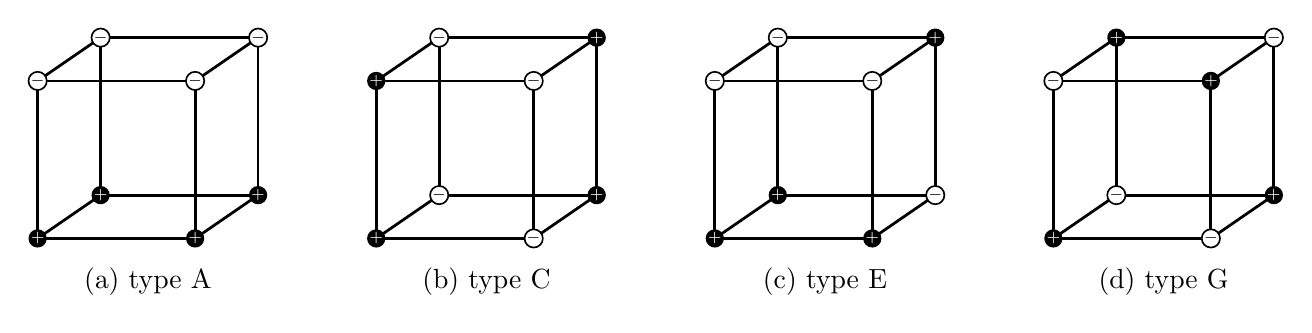
\begin{tikzpicture}[line width=0.8pt,>=Stealth]
\begin{scope}[shift={(0,0)}]
  \mcube{-1}{-1}{-1}{-1}{1}{1}{1}{1}
  \node at (1.4,-0.55) {(a) type A};
\end{scope}
\begin{scope}[shift={(4.3,0)}]
  \mcube{1}{-1}{-1}{1}{1}{-1}{-1}{1}
  \node at (1.4,-0.55) {(b) type C};
\end{scope}
\begin{scope}[shift={(8.6,0)}]
  \mcube{-1}{-1}{-1}{1}{1}{1}{1}{-1}
  \node at (1.4,-0.55) {(c) type E};
\end{scope}
\begin{scope}[shift={(12.9,0)}]
  \mcube{-1}{1}{1}{-1}{1}{-1}{-1}{1}
  \node at (1.4,-0.55) {(d) type G};
\end{scope}
\end{tikzpicture}
\end{document}
